\documentclass[tikz]{standalone}
\usepackage{amsmath}

\begin{document}

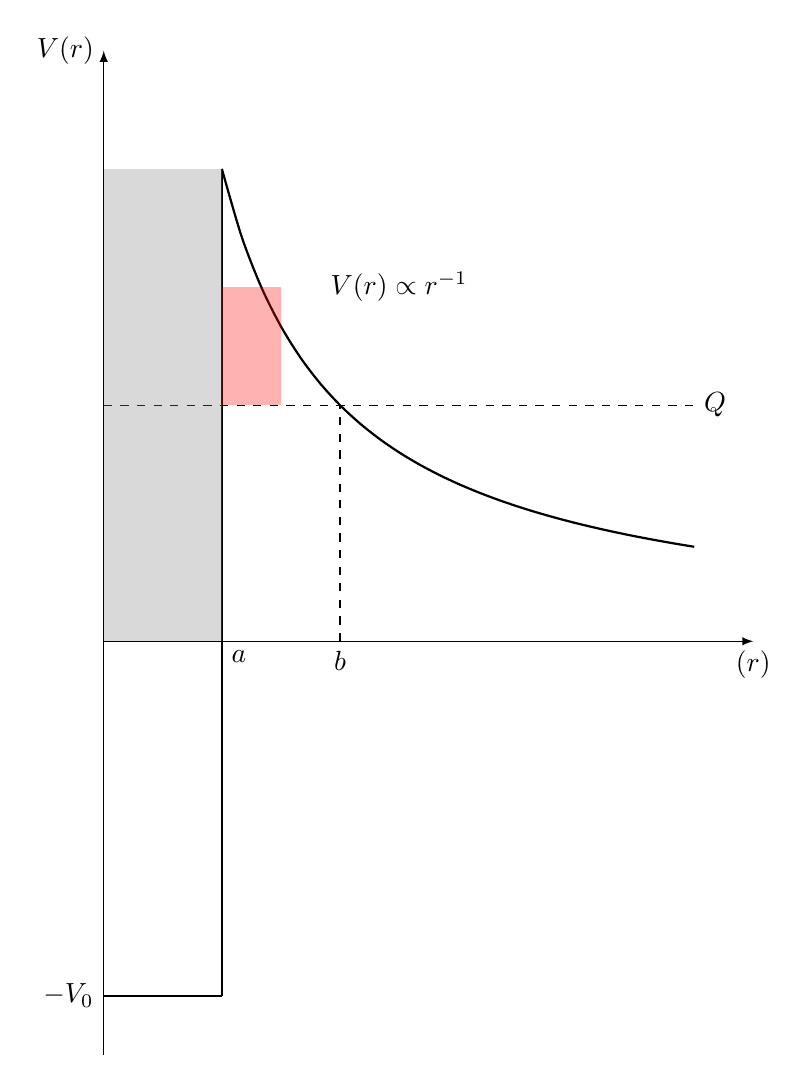
\begin{tikzpicture}[scale=1.5, >=latex]

% Ejes
\draw[->] (0, 0) -- (5.5, 0) node[anchor=north] { ($r$)};
\draw[->] (0, -3.5) -- (0, 5) node[anchor=east] {$V(r)$};

% Barrera de Coulomb
\draw[thick, domain=1:5, smooth, variable=\x] plot (\x, {4/(\x)}) node[anchor=south] {};
\draw[thick] (1, 4) -- (1, -3);
\draw[thick] (0, -3) node[left]{$-V_0$} -- (1, -3);
% Energía de la partícula alfa
\draw[dashed] (0, 2) -- (5, 2) node[anchor=west] {$Q$};
\draw[dashed] (2, 0) -- (2, 2);
\fill[gray,opacity=0.3] (0,0) rectangle (1,4);
\fill[red,opacity=0.3] (1,2) rectangle (1.5,3);
% Etiquetas
\node at (2.5, 3) {$V(r)\propto r^{-1}$};
\node[below right] at (1, 0) {$a$};
\node [below] at (2, 0) {$b$};

\end{tikzpicture}

\end{document}
